

\documentclass{beamer}

\usepackage[T1]{fontenc}
\usepackage[utf8]{inputenc}
\usepackage[french,english]{babel}

\usepackage{lmodern}
\usepackage{amsthm}
\usepackage{float}
\usepackage{lmodern}%pour un meilleur rendu des polices
\usepackage{verbatim}%du texte non interprt
\usepackage{amsmath}
\usepackage{amssymb}%maths
\usepackage{xspace}
\usepackage[dvipsnames,svgnames,table]{xcolor}
\usepackage{listings}
\usepackage{fancyhdr}
\usepackage{etoolbox}
\usepackage{titlesec}
\usepackage{titletoc}
\usepackage{lastpage}
\usepackage{hyperref}
\usepackage{ctable} % for \specialrule command
\usepackage{cite}
\usepackage{algorithm2e}
\usepackage{alltt}
\usepackage{array}
\usepackage{mdwmath}
\usepackage{mdwtab}
\usepackage{eqparbox}
\usepackage{subfig}
\usepackage{dblfloatfix}
\usepackage{url}
\usepackage{tipa}
\usepackage{stmaryrd}
\usepackage{upgreek}
\usepackage{mathrsfs}
\usepackage{ulem}
\usepackage{cancel}

\graphicspath{{img/}}
\DeclareGraphicsExtensions{.pdf,.jpeg,.jpg,.png}


\newcommand{\ccite}[1]{\textbf{\cite{#1}}}
\newcommand{\pd}[2]{\dfrac{\partial #1}{\partial #2}}
\newcommand{\od}[2]{\dfrac{\mathscr{D}_a #1}{\mathscr{D} #2}}
\newcommand{\tensor}[1]{\mathbf{#1}}
\renewcommand{\vector}[1]{\overrightarrow{#1}}

\newcommand{\Tau}{\tensor{\mathlarger{\uptau}}}
\renewcommand{\v}{\vector{u}}
\newcommand{\W}{\tensor{W\left( \v \right)}}
\newcommand{\D}{\tensor{D\left( \v \right)}}
\newcommand{\grad}{\vector{\nabla}}
\newcommand{\gradv}{\tensor{\nabla\v}}
\renewcommand{\div}[1]{div \left( #1 \right)}
\newcommand{\divv}[1]{\vector{div} \left( #1 \right)}
\newcommand{\UU}{\mathcal{U}}
\newcommand{\VV}{\mathcal{U}}
\newcommand{\M}{\mathcal{M}}
\newcommand{\A}[2]{\mathcal{A}_{#1}\left( #2 \right)}
\newcommand{\Uu}{\UU^{n}}
\newcommand{\Uv}{\UU^{n+\theta}}
\newcommand{\Uw}{\UU^{n+1-\theta}}
\newcommand{\Ux}{\UU^{n+1}}
\newcommand{\Uk}{\UU^{k}}
\newcommand{\Ukk}{\UU^{k+1}}
\newcommand{\Vk}{\VV^{k}}
\newcommand{\Vkk}{\VV^{k+1}}
\newcommand{\Tauk}{\Tau^{k+1}}
\newcommand{\vk}{\v^{k+1}}
\newcommand{\pk}{p^{k+1}}
\newcommand{\Dk}{\tensor{D\left( \vk \right)}}

\definecolor{lightgray}{gray}{0.9}
\definecolor{titlecolor}{RGB}{0,0,200}
\definecolor{subtitlecolor}{RGB}{0,0,153}
\definecolor{textcolor}{RGB}{0,128,255}
\definecolor{RoyalPurple}{RGB}{102,51,153}
\definecolor{ForestGreen}{RGB}{34,139,34}


\newcommand{\colbox}[1]{\colorbox{lightgray}{$ #1 $}}

\newcommand{\stitle}[2][0.3cm] { 
    {\normalsize \textcolor{titlecolor}{\textbf{#2}}} 
    \vspace{#1} 
}

\newcommand{\ssubtitle}[1]{ {\footnotesize \textcolor{subtitlecolor}{\textbf{#1}}} }

\newcommand{\stress}[1]{\textcolor{textcolor}{#1}}

\newcommand{\hidecontent}[2][0.25]{{% \hidecontent[<transparency>]{<stuff>}
  \setbox9=\hbox{#2}% Store <stuff> in \box9 to obtain height/width
  \transparent{#1}\ooalign{\usebox9\cr\color{white}\rule{\wd9}{\ht9}\cr}}}



\usetheme{Frankfurt}
\def\beamertemplatetransparentcoveredmedium{\setbeamercovered{transparent=40}}
\def\beamertemplatetransparentcoveredhard{\setbeamercovered{transparent=20}}
\beamertemplatetransparentcoveredmedium
\setbeamertemplate{bibliography item}[triangle]
\addtobeamertemplate{footline}{\hfill\insertframenumber/\inserttotalframenumber\hspace{2em}\null}

\begin{document}


\title{\Large A new operator splitting algorithm for elastoviscoplastic flow problems}
\author[Keck]{\Large Jean-Baptiste Keck}
\institute[MSIAM]{\Large \bsc{M2 Msiam}}
\date{\large Paper Review\\ 06/02/2015}



\begin{frame}
    \titlepage
\end{frame}


\begin{frame}{Operator notations} 

    \stitle{Operators :}
    \tiny

\uncover<1>{
$
\begin{array}{l l l c c l c l c}
    \gradv& = & 

    \underbrace{\D}_{{\only<1>{\color{red}}deformation\ rate}}& + & \underbrace{\W}_{{\only<1>{\color{textcolor}}{vorticity}}}& = &
    \left[\dfrac{\gradv + \gradv^T}{2}\right]& + & \left[\dfrac{\gradv - \gradv^T}{2}\right] \\
\end{array}
$
}
    
\\

\uncover<2>{
$
\begin{array}{l l l c c l c l c}
    \Tau & = & \underbrace{\Tau_d}_{\underset{(shear)}{{\only<2>{\color{red}}deviatoric\ stress}}}& + & \underbrace{\Tau_s}_{\underset{(pressure)}{{\only<2>{\color{textcolor}}hydrostatic\ stress}}} &
    = & \left[\Tau - \dfrac{1}{d}tr(\Tau)\tensor{I_d}\right]& + & \left[\dfrac{1}{d}tr(\Tau)\tensor{I_d}\right]
\end{array}
$
}
    
\vskip 0.5cm

\uncover<3>{
$
\forall a \in \left[ -1,1\right] \hspace{0.5cm}
\tensor{{\only<3>{\color{textcolor}}\od{\Tau}{t}}} = \pd{\Tau}{t} + \left(\v . \grad \right) \Tau + \tensor{{\only<3>{\color{red}}\beta_a} \left( \Tau, \gradv \right)}
\textrm{\ \ the {\only<3>{\color{textcolor}} \textbf{Jaumann objective stress rate.}}}
$
\vskip 0.5cm
$
\hskip 2.6cm
{\only<3>{\color{red}}\beta_a} \left( \Tau, \gradv \right) = \Tau . \W - \W . \Tau - a \left[ \D.\Tau + \Tau . \D \right]
$
}

\vskip 0.5cm

\uncover<4>{
$
\forall \; \Tau \in \mathbb{R}^{d \times d} \hskip 0.5cm
{\only<4>{\color{red}}|\Tau|^2}=
\Tau : \Tau =
tr\left(\Tau^T \Tau \right) =
\sum_{1\leq i,j \leq d}\Tau_{ij}^2 \hskip 0.5cm \textrm{ the usual {\only<4>{\color{textcolor}}\textbf{matrix Euclidean norm}}}
$
}

\end{frame}


\begin{frame}{\normalsize Model parameters and notations} 

\stitle{Model parameters}
\footnotesize

\uncover<1-6>{
\ssubtitle{Dimension: } $d \in \left\{ 2,3\right\}$
}
\vskip 0.2cm
\uncover<2-6>{
\ssubtitle{Jaumann operator parameter: } $a \in \left[-1,1\right]$
}
\vskip 0.2cm
\uncover<3-6>{
\ssubtitle{Fluid properties:}
\vskip 0.3cm
    \tiny

$
\left[
\begin{array}{l l}
    \rho &solution\ density&
    \eta_s &solvent\ \ viscosity&
    \eta_m &polymer\ viscosity&
    \lambda &elastic\ relaxation\ time&
    \Tau_Y &yield\ stress&
\end{array}
\right]
$
\only<4-6>{
$
\Leftrightarrow
\left[
\begin{array}{l l l l}
    L,V&=&\multicolumn{2}{l}{Caracteristic\ length\ and\ velocity}&
    W_e&=& \lambda V/L &Weissenberg\ number&
    B_i&=& \Tau_YL/\eta_m &Bingham\ number&
    R_e&=& \rho VL/(\eta_m+\eta_s) &Reynolds\ number&
    \alpha&=&\eta_m/(\eta_m+\eta_s) &Retardation\ parameter&
\end{array}
\right]
$
}
}

\vskip 0.5cm

\uncover<5-6>{
\stitle{Additional notations}
}
\footnotesize

\uncover<5-6>{
\ssubtitle{Cauchy stress tensor:} $\Tau_{tot} = \underbrace{\Tau}_{elastic\ stress} - \underbrace{p\tensor{Id}}_{pressure} + \underbrace{2\eta_s\D}_{viscous\ friction}$
}


\uncover<6>{
\ssubtitle{Yield response:} $\mathcal{K}(|\alert{\Tau_d}|) = \left[ \dfrac{|\Tau_d| - Bi}{n |\Tau_d|}\right]_+^n = \textrm{\textbf{max}}\left(0, \; 1 - \dfrac{B_i}{|\Tau_d|} \right) \textrm{ with } n = 1 \textrm{ (Bingham)}.$\\
\vskip 0.1cm
\indent\hskip 1.5cm \alert{$\Tau_d$} is the \stress{elastic shear stress}
}

\end{frame}


\begin{frame}{Domain}

    \stitle[0.0cm]{Experimental configuration :}
    \footnotesize

\begin{table}[h]
    \centering
    $
    \begin{array}{l c c c c c r}
        \mathlarger{\Omega \subset \mathbb{R}^d} &
        &&   
        \mathlarger{\partial\Omega = \textcolor{ForestGreen}{\Gamma_d} \cup \textcolor{blue}{\Gamma_n} \cup \alert{\Gamma_s}} &
        &&
        \underbrace{\partial\Omega_- = \Gamma_- = \left\{x\in \partial\Omega\ |\ \v.\vector{n} < 0\right\}}_{upstream\ boundary} 
    \end{array}
    $
\end{table}

\begin{figure}[h!]
   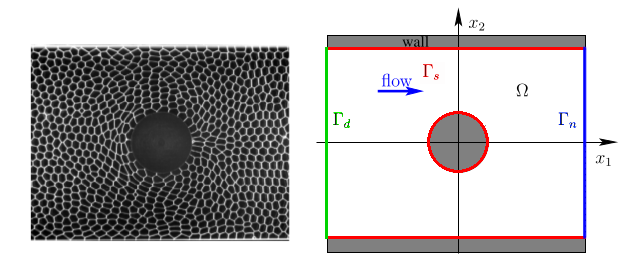
\includegraphics[scale=0.5]{domain.png}
\end{figure}

\end{frame}



\begin{frame}{Model}

\setbeamercovered{invisible}
\scriptsize
Find $\stress{\ \mathcal{U}} = (\Tau,\v, p)^T : \; \left]0,T\right[ \times \Omega \rightarrow \mathbb{R}^{d\times d} \times \mathbb{R}^d \times \mathbb{R}$ such that :

\vfill
$
   \left\{
       \begin{array}{l l l l}
           
           (1)& 
           W_e\left[\textcolor{blue}{\tensor{\od{\Tau}{t}}}\right] 
           
           + {\tiny \only<2->{\color{red}} \uncover<2->{\underbrace{\mathcal{K} \left( | \Tau_d | \right)}_{plastic\ dissipation}} \Tau} - 2\alpha \tensor{D(\v)}&
           =& 0_{\mathbb{R}^{d \times d}} \\
           
           \\

           (2)&
           R_e\left[ \pd{\v}{t} + \textcolor{RoyalPurple}{
                   \only<3->{\cancel}{\left(\v . \grad \right) \v}
           } \right] 
           \underbrace{-\divv{\Tau -p\tensor{I}_d+2\eta_s\tensor{D(\v)}}}_{ -\divv{\Tau_{tot}} = -\divv{\Tau} + \grad p - (1-\alpha)\Delta\v}&
           =& 0_{\mathbb{R}^d} \\

           (3)& \div{\v} &=& 0_\mathbb{R} \\

           \\

           \uncover<4>{
           (4)& 
           \multicolumn{3}{l}{
           \v = \vector{v_{\Gamma_d}} \hskip 0.58cm \textrm{ in } ]0,T[\ \times\ \Gamma_d
           \hskip 2.4cm \v . \vector{n} = 0\textrm{ in } ]0,T[ \times \Gamma_s
           } \\
           
           (5)&
           \multicolumn{3}{l}{
           \vector{F} = \Tau \vector{n} = 0 \textrm{ in } \left]0,T\right[ \times \Gamma_n
           \hskip 0.9cm 
           \vector{F_t} = \Tau \vector{n} - \Tau_{nn} \vector{n} = 0 \textrm{ in } ]0,T[ \times \Gamma_s
           } \\

           (6)&
           \multicolumn{3}{l}{
           \Tau = \Tau_- \hskip 0.775cm \textrm{ in } \left]0,T\right[ \times \Gamma_-
           } \\
        }
       \end{array}
   \right.
$
\vfill

\end{frame}


\begin{frame}{Operator Splitting}

\beamertemplatetransparentcoveredhard

\ssubtitle{Rewrite the model as:}
\scriptsize
\vskip 0.5cm

Find $\ \stress{\mathcal{U}} = (\Tau,\v, p)^T : \; \left]0,T\right[ \times \Omega \rightarrow \mathbb{R}^{d\times d} \times \mathbb{R}^d \times \mathbb{R}$ such that :

\vskip 0.3cm
\hskip 1.3cm
    $
    \left\{
        \begin{array}{l}
            \M \pd{\UU}{t} + \A{}{\UU}= 0_{\mathbb{R}^{d\times d}\times \mathbb{R}^d \times \mathbb{R}} &
            &
            (4) \hskip 0.5cm (5) \hskip 0.5cm (6) \hskip 0.5cm \textrm{(Boundary conditions)}
        \end{array}
    \right.
    $

        \vskip 0.5cm
\hskip 1.0cm with $\M =
    \left [
       \begin{array}{c c c}
           W_e&0&0&
           0&R_e&0&
           0&0&0&
       \end{array}
    \right ]
    \textrm{ and } \A{}{\UU} =  \alert{\A{1}{\UU}} + \textcolor{blue}{\A{2}{\UU}}
$

\vskip 0.5cm
$$
\A{}{\UU} = 
\uncover<2->{
\underbrace{
    \left[\begin{array}{c}
            \textcolor{red}{\mathcal{K} \left( | \Tau_d | \right) \Tau} - 2\alpha \tensor{D(\v)}&
            -\divv{\Tau} + \grad p - (1-\alpha)\Delta\v&
            \div{\v}&
\end{array}\right]}_{\alert{\A{1}{\UU}}\ contains\ all\ \alert{viscoplastic\ effects}}
}
+
\uncover<3->{
\underbrace{
    \left[\begin{array}{c}
           W_e\left[\textcolor{blue}{\left(\v . \grad \right) \Tau + \tensor{\beta_a \left( \Tau, \gradv \right)}}\right]&
           0&
           0&
\end{array}\right]}_{\textcolor{blue}{\A{2}{\UU}}\ contains\ all\ \textcolor{blue}{viscoelastic\ effects}}
}
$$

\end{frame}


\begin{frame}{$\Theta$-Scheme}

    \scriptsize
\ssubtitle{Three-steps $\theta$-scheme time-approximation of the previous equation :}

\vskip 0.5cm
Let $\Delta t > 0$ and $\theta \in \left] 0,1/2 \right[$ and $\UU_n$ be given. 
    
    \vskip 0.2cm
    \textbf{To compute } \textcolor{blue}{$\mathbf{\UU_{n+1}}$} \textbf{compute successively the following subproblems} :

    \tiny
$$
\begin{array}{l c c c l c l c r}
    \alert{\mathcal{P}_1}\left(\textcolor{blue}{\Uv},\Uu\right)&\Leftrightarrow&
    \M\dfrac{\textcolor{blue}{\Uv} - \Uu}{\theta \Delta t}&+&\A{1}{\textcolor{blue}{\Uv}}&+&\A{2}{\Uu}&=&0\\
    \\
    \alert{\mathcal{P}_2}\left(\textcolor{blue}{\Uw},\Uv\right)&\Leftrightarrow&
    \M\dfrac{\textcolor{blue}{\Uw} - \Uv}{(1-2\theta) \Delta t}&+&\A{1}{\Uv}&+&\A{2}{\textcolor{blue}{\Uw}}&=&0\\
    \\
    \alert{\mathcal{P}_1}\left(\textcolor{blue}{\Ux},\Uw\right)&\Leftrightarrow&
    \M\dfrac{\textcolor{blue}{\Ux} - \Uw}{\theta \Delta t}&+&\A{1}{\textcolor{blue}{\Ux}}&+&\A{2}{\Uw}&=&0
\end{array}
$$

\begin{figure}[h!]
   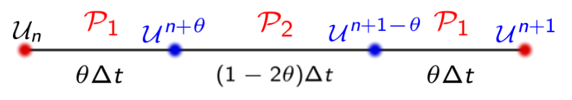
\includegraphics[scale=0.35]{scheme.png}
\end{figure}

    \scriptsize
    \stress{The third step is similar to the first one.}

\end{frame}



\begin{frame}{First subproblem}
    \stitle{Solving the first subproblem $\mathcal{P}_1$ :}

\scriptsize
Let $\Uk = \left[ \Tau^k, \v^k, p^k \right]^T$ be given. \alert{$\mathcal{P}_1$} is a \textbf{non linear Stokes problem} :

\vskip 0.3cm
\hskip 0.5cm
$\mathcal{P}_1\left(\textcolor{blue}{\Ukk},\Uk\right)
\hskip 0.5cm
\Leftrightarrow
\hskip 0.5cm
\M\dfrac{\textcolor{blue}{\Ukk}}{\theta \Delta t}+\A{1}{\textcolor{blue}{\Ukk}} = \mathcal{M}\dfrac{\Uk}{\theta \Delta t} - \A{2}{\Uk} = \mathcal{V}^k

\vskip 0.5cm
\Leftrightarrow
\left\{
    \begin{array}{l c l}
        W_e\dfrac{\Tau^{k+1}}{\theta\Delta t} + \textcolor{red}{\mathcal{K} \left( | \Tau_d^{k+1} | \right) \Tauk} - 2\alpha \Dk&=&\mathcal{V}^k_1\\
        \\
        Re\dfrac{\vk}{\theta\Delta t}-\divv{\Tauk} + \grad \pk - (1-\alpha)\Delta\vk&=&\mathcal{V}^k_2\\
        \\
        \div{\vk}&=&0
    \end{array}
\right .
$

\end{frame}

\begin{frame}{Linearizing the first subproblem}
    \scriptsize

    \stitle{\textbf{Fixed point algorithm :}}

Linearize problem $\mathcal{P}_1$ with $\textcolor{red}{\mathcal{K} \left( | \Tau_d^{k+1} | \right) \Tauk} \simeq \underbrace{\mathcal{K} \left( \textcolor{RoyalPurple}{| \Tau_d^{k} |} \right)}_{explicit} \Tauk 
\\
\Rightarrow \mathcal{P}_1^{\alert{lin}}$ becomes a {\scriptsize\stress{"\textbf{simple Stokes subproblem}"}}

\vskip 0.5cm

\ssubtitle{Step $\mathbf{s = 0}$:} 
Let $\textcolor{blue}{\UU^k_0} = \UU^k
\hspace{1.1cm} i.e. \hspace{0.5cm}
\left(\Tau^k_0, \v^k_0, p^k_0\right) = \left(\Tau^k, \v^k, p^k\right)$

\vskip 0.3cm
\ssubtitle{Step $\mathbf{s > 0}$:} 
Solve $\mathcal{P}_1^{\alert{lin}} 
\left( \textcolor{blue}{\UU^k_{s+1}}, \UU^k_s \right)$ with boundary conditions (4-5) to compute $\textcolor{blue}{\UU^k_{s+1}}$ .
\vskip 0.2cm
\ssubtitle{Finally :}
\hspace{0.3cm}
Set $\textcolor{blue}{\Ukk} = \UU^k_{s_{\infty}} 
\hspace{0.5cm} i.e. \hspace{0.5cm}
\left(\Tauk, \vk, \pk\right) =
\left(\Tau^k_{s_{\infty}}, \v^k_{s_{\infty}}, p^k_{s_{\infty}}\right)$

\end{frame}



\begin{frame}{Second subproblem}

\stitle{Solving the second subproblem $\mathcal{P}_2$}
    \scriptsize

    Let $\Vk = \left[ \Tau^k, \v^k, p^k \right]^T$ and $\theta'=1-2\theta$ be given. \alert{$\mathcal{P}_2$} is a \textbf{stress transport problem} :

\vskip 0.3cm
$\mathcal{P}_2\left(\textcolor{blue}{\Vkk},\Vk\right)
\hskip 0.5cm
\Leftrightarrow
\hskip 0.5cm
\M\dfrac{\textcolor{blue}{\Vkk}}{\theta' \Delta t}+\A{2}{\textcolor{blue}{\Vkk}} = \mathcal{M}\dfrac{\Vk}{\theta' \Delta t} - \A{1}{\Vk} = \mathcal{W}^k

\vskip 0.5cm
\Leftrightarrow
\left\{
    \begin{array}{l c l}
        \dfrac{\Tauk}{\theta'\Delta t} + \textcolor{blue}{\left(\v^{k+1} . \grad \right) \Tau^{k+1} + \tensor{\beta_a \left( \Tau^{k+1}, \gradv^{k+1} \right)}}&=&\mathcal{W}^k_1\\
        \\
        Re\dfrac{\vk}{\theta'\Delta t}=
        Re\dfrac{\v^k}{\theta'\Delta t}+\divv{\Tau^k} - \grad p^k + (1-\alpha)\Delta\v^k
        &=&\mathcal{W}_2^k
    \end{array}
\right .
$

\vskip 0.5cm
\textbf{If we previously have solved} $\mathbf{\mathcal{P}_1 \left(\UU^k, \UU^{k-1}\right)}$ \textbf{:}
%\vskip 0.2cm
%$\mathcal{W}_2^k 
%= Re\left[\dfrac{\v^{k}}{\theta'\Delta t} + \dfrac{\v^{k}}{\theta\Delta t}\right] - \mathcal{V}^k_2
%= Re\left[\dfrac{\v^{k}}{\theta'\Delta t} + \dfrac{\v^{k}}{\theta\Delta t} +  \dfrac{\v^{k-1}}{\theta\Delta t} \right]
\alert{\vk}=\underbrace{\dfrac{1-\theta}{\theta}\v^k -  \dfrac{1-2\theta}{\theta}\v^{k-1}}_{explicit}$

$\Rightarrow \alert{\mathcal{P}_2}$ becomes a \stress{\textbf{linear Friedrich’s first-order system}}.

\vskip 0.2cm
It admits a solution if $\Delta t < \dfrac{1}{\theta'} - 2\ |a|\  ||\tensor{D(\v^k)}||_\infty$
 
\end{frame}




%\begin{frame}{References}
    %\raggedright
    %\nocite{*}
    %\bibliographystyle{plain}
    %\bibliography{master}
    %\vfill
    %\begin{center}
        %\Large
        %Any questions ?
    %\end{center} 
%\end{frame}

\end{document}
